% !TEX root = aula01.tex
% ============================================================
%  TEMPLATE BEAMER --- Tema "Dark Accent"
% ============================================================
%  Este arquivo concentra TODO o preâmbulo compartilhado entre
%  as aulas (classe do documento, pacotes, cores, fontes,
%  cabeçalho/rodapé dos slides e comandos auxiliares).
%
%  Como usar em um novo arquivo de aula:
%
%      % ============================================================
%  TEMPLATE BEAMER --- Tema "Dark Accent"
% ============================================================
%  Este arquivo concentra TODO o preâmbulo compartilhado entre
%  as aulas (classe do documento, pacotes, cores, fontes,
%  cabeçalho/rodapé dos slides e comandos auxiliares).
%
%  Como usar em um novo arquivo de aula:
%
%      % ============================================================
%  TEMPLATE BEAMER --- Tema "Dark Accent"
% ============================================================
%  Este arquivo concentra TODO o preâmbulo compartilhado entre
%  as aulas (classe do documento, pacotes, cores, fontes,
%  cabeçalho/rodapé dos slides e comandos auxiliares).
%
%  Como usar em um novo arquivo de aula:
%
%      \input{templates/beamer.tex}
%
%      \title{Título da Aula}
%      \author
%
%      \begin{document}
%        ... seus \begin{frame} ... \end{frame} ...
%      \end{document}
%
%  IMPORTANTE: como este arquivo contém o \documentclass, ele
%  precisa ser a PRIMEIRA linha do .tex da aula (nenhum outro
%  comando pode vir antes do \input acima).
%
%  Compilar sempre a partir da pasta latex/ (para o caminho
%  relativo "templates/beamer.tex" ser encontrado):
%      cd latex && pdflatex aula01.tex
% ============================================================

% !TEX root = ../aula01.tex

\documentclass[11pt, aspectratio=169, xcolor=table]{beamer}

% ===================== PACOTES =====================
\usepackage[utf8]{inputenc}
\usepackage[T1]{fontenc}
\usepackage{lmodern}
\usepackage{newtxtext}
\usepackage{newtxmath}
\usepackage{tikz}
\usepackage{amsmath, amssymb}
\usepackage{booktabs}
\usepackage{bookmark}

% Atalho para "d" reto de diferenciais: dx, dy -> \dd x, \dd y
\newcommand{\dd}{\mathrm{d}}

% ===================== REMOVE ELEMENTOS PADRÃO DO BEAMER =====================
\setbeamertemplate{navigation symbols}{}

% ===================== CORES =====================
\definecolor{bgcolor}{RGB}{20, 20, 24}
\definecolor{accent}{RGB}{214, 165, 113}
\definecolor{dotoff}{RGB}{70, 70, 76}

\setbeamercolor{background canvas}{bg=bgcolor}
\setbeamercolor{normal text}{fg=white!92!black}
\setbeamercolor{title}{fg=white}
\setbeamercolor{frametitle}{fg=accent}
\setbeamercolor{footline}{fg=gray!60}
\setbeamercolor{itemize item}{fg=accent}
\setbeamercolor{itemize subitem}{fg=accent!70!white}
\setbeamercolor{progress}{bg=bgcolor}
\setbeamercolor{footnum}{bg=bgcolor}
\setbeamertemplate{itemize item}{\textbullet}

\setbeamerfont{frametitle}{series=\bfseries}
\setbeamerfont{footline}{size=\tiny}

\hypersetup{colorlinks=true, urlcolor=accent, linkcolor=accent}

% ===================== TÍTULO DO SLIDE =====================
\setbeamertemplate{frametitle}{
  \vspace{0.5cm}
  \hspace{0.4cm}\usebeamerfont{frametitle}\usebeamercolor[fg]{frametitle}\insertframetitle\\
  \vspace{0.12cm}
  \hspace{0.4cm}\textcolor{accent}{\rule{2.5cm}{0.6pt}}
}

% ===================== RODAPÉ =====================
\setbeamertemplate{footline}{%
  \begin{beamercolorbox}[wd=\paperwidth, ht=0.09cm, dp=0pt]{progress}
    \begin{tikzpicture}
      \fill[dotoff] (0,0) rectangle (16,0.09);
      \ifnum\inserttotalframenumber>0
        \pgfmathsetmacro{\prog}{16*\insertframenumber/\inserttotalframenumber}
        \fill[accent] (0,0) rectangle (\prog,0.09);
      \fi
    \end{tikzpicture}
  \end{beamercolorbox}%
  \vskip 2pt
  \begin{beamercolorbox}[wd=\paperwidth, ht=2.4ex, dp=1.2ex, right]{footnum}
    \usebeamerfont{footline}\color{gray!60}\insertframenumber\,/\,\inserttotalframenumber\hspace{0.8em}
  \end{beamercolorbox}%
}

\setlength{\parindent}{0pt}
\setlength{\parskip}{6pt}

% ===================== CUSTOMIZAÇÃO DE BLOCOS =====================
\setbeamertemplate{blocks}[rounded][shadow=false]
\setbeamercolor{block title}{bg=dotoff, fg=accent}
\setbeamercolor{block body}{bg=bgcolor!90!white, fg=white!92!black}

\setbeamercolor{block title alerted}{bg=accent!60!black, fg=white}
\setbeamercolor{block body alerted}{bg=bgcolor!95!white, fg=white!92!black}

% ===================== CAIXA DE DESTAQUE =====================
% Uso: \notebox{texto da observação}
\newcommand{\notebox}[1]{%
  \begin{center}
  \begin{tabular}{@{}l@{\hspace{0.35cm}}p{0.82\textwidth}@{}}
    \textcolor{accent}{\rule{2pt}{0.55cm}} & \itshape\small\color{white!88!black} #1
  \end{tabular}
  \end{center}%
}

\usefonttheme[onlymath]{serif}
%
%      \title{Título da Aula}
%      \author
%
%      \begin{document}
%        ... seus \begin{frame} ... \end{frame} ...
%      \end{document}
%
%  IMPORTANTE: como este arquivo contém o \documentclass, ele
%  precisa ser a PRIMEIRA linha do .tex da aula (nenhum outro
%  comando pode vir antes do \input acima).
%
%  Compilar sempre a partir da pasta latex/ (para o caminho
%  relativo "templates/beamer.tex" ser encontrado):
%      cd latex && pdflatex aula01.tex
% ============================================================

% !TEX root = ../aula01.tex

\documentclass[11pt, aspectratio=169, xcolor=table]{beamer}

% ===================== PACOTES =====================
\usepackage[utf8]{inputenc}
\usepackage[T1]{fontenc}
\usepackage{lmodern}
\usepackage{newtxtext}
\usepackage{newtxmath}
\usepackage{tikz}
\usepackage{amsmath, amssymb}
\usepackage{booktabs}
\usepackage{bookmark}

% Atalho para "d" reto de diferenciais: dx, dy -> \dd x, \dd y
\newcommand{\dd}{\mathrm{d}}

% ===================== REMOVE ELEMENTOS PADRÃO DO BEAMER =====================
\setbeamertemplate{navigation symbols}{}

% ===================== CORES =====================
\definecolor{bgcolor}{RGB}{20, 20, 24}
\definecolor{accent}{RGB}{214, 165, 113}
\definecolor{dotoff}{RGB}{70, 70, 76}

\setbeamercolor{background canvas}{bg=bgcolor}
\setbeamercolor{normal text}{fg=white!92!black}
\setbeamercolor{title}{fg=white}
\setbeamercolor{frametitle}{fg=accent}
\setbeamercolor{footline}{fg=gray!60}
\setbeamercolor{itemize item}{fg=accent}
\setbeamercolor{itemize subitem}{fg=accent!70!white}
\setbeamercolor{progress}{bg=bgcolor}
\setbeamercolor{footnum}{bg=bgcolor}
\setbeamertemplate{itemize item}{\textbullet}

\setbeamerfont{frametitle}{series=\bfseries}
\setbeamerfont{footline}{size=\tiny}

\hypersetup{colorlinks=true, urlcolor=accent, linkcolor=accent}

% ===================== TÍTULO DO SLIDE =====================
\setbeamertemplate{frametitle}{
  \vspace{0.5cm}
  \hspace{0.4cm}\usebeamerfont{frametitle}\usebeamercolor[fg]{frametitle}\insertframetitle\\
  \vspace{0.12cm}
  \hspace{0.4cm}\textcolor{accent}{\rule{2.5cm}{0.6pt}}
}

% ===================== RODAPÉ =====================
\setbeamertemplate{footline}{%
  \begin{beamercolorbox}[wd=\paperwidth, ht=0.09cm, dp=0pt]{progress}
    \begin{tikzpicture}
      \fill[dotoff] (0,0) rectangle (16,0.09);
      \ifnum\inserttotalframenumber>0
        \pgfmathsetmacro{\prog}{16*\insertframenumber/\inserttotalframenumber}
        \fill[accent] (0,0) rectangle (\prog,0.09);
      \fi
    \end{tikzpicture}
  \end{beamercolorbox}%
  \vskip 2pt
  \begin{beamercolorbox}[wd=\paperwidth, ht=2.4ex, dp=1.2ex, right]{footnum}
    \usebeamerfont{footline}\color{gray!60}\insertframenumber\,/\,\inserttotalframenumber\hspace{0.8em}
  \end{beamercolorbox}%
}

\setlength{\parindent}{0pt}
\setlength{\parskip}{6pt}

% ===================== CUSTOMIZAÇÃO DE BLOCOS =====================
\setbeamertemplate{blocks}[rounded][shadow=false]
\setbeamercolor{block title}{bg=dotoff, fg=accent}
\setbeamercolor{block body}{bg=bgcolor!90!white, fg=white!92!black}

\setbeamercolor{block title alerted}{bg=accent!60!black, fg=white}
\setbeamercolor{block body alerted}{bg=bgcolor!95!white, fg=white!92!black}

% ===================== CAIXA DE DESTAQUE =====================
% Uso: \notebox{texto da observação}
\newcommand{\notebox}[1]{%
  \begin{center}
  \begin{tabular}{@{}l@{\hspace{0.35cm}}p{0.82\textwidth}@{}}
    \textcolor{accent}{\rule{2pt}{0.55cm}} & \itshape\small\color{white!88!black} #1
  \end{tabular}
  \end{center}%
}

\usefonttheme[onlymath]{serif}
%
%      \title{Título da Aula}
%      \author
%
%      \begin{document}
%        ... seus \begin{frame} ... \end{frame} ...
%      \end{document}
%
%  IMPORTANTE: como este arquivo contém o \documentclass, ele
%  precisa ser a PRIMEIRA linha do .tex da aula (nenhum outro
%  comando pode vir antes do \input acima).
%
%  Compilar sempre a partir da pasta latex/ (para o caminho
%  relativo "templates/beamer.tex" ser encontrado):
%      cd latex && pdflatex aula01.tex
% ============================================================

% !TEX root = ../aula01.tex

\documentclass[11pt, aspectratio=169, xcolor=table]{beamer}

% ===================== PACOTES =====================
\usepackage[utf8]{inputenc}
\usepackage[T1]{fontenc}
\usepackage{lmodern}
\usepackage{newtxtext}
\usepackage{newtxmath}
\usepackage{tikz}
\usepackage{amsmath, amssymb}
\usepackage{booktabs}
\usepackage{bookmark}

% Atalho para "d" reto de diferenciais: dx, dy -> \dd x, \dd y
\newcommand{\dd}{\mathrm{d}}

% ===================== REMOVE ELEMENTOS PADRÃO DO BEAMER =====================
\setbeamertemplate{navigation symbols}{}

% ===================== CORES =====================
\definecolor{bgcolor}{RGB}{20, 20, 24}
\definecolor{accent}{RGB}{214, 165, 113}
\definecolor{dotoff}{RGB}{70, 70, 76}

\setbeamercolor{background canvas}{bg=bgcolor}
\setbeamercolor{normal text}{fg=white!92!black}
\setbeamercolor{title}{fg=white}
\setbeamercolor{frametitle}{fg=accent}
\setbeamercolor{footline}{fg=gray!60}
\setbeamercolor{itemize item}{fg=accent}
\setbeamercolor{itemize subitem}{fg=accent!70!white}
\setbeamercolor{progress}{bg=bgcolor}
\setbeamercolor{footnum}{bg=bgcolor}
\setbeamertemplate{itemize item}{\textbullet}

\setbeamerfont{frametitle}{series=\bfseries}
\setbeamerfont{footline}{size=\tiny}

\hypersetup{colorlinks=true, urlcolor=accent, linkcolor=accent}

% ===================== TÍTULO DO SLIDE =====================
\setbeamertemplate{frametitle}{
  \vspace{0.5cm}
  \hspace{0.4cm}\usebeamerfont{frametitle}\usebeamercolor[fg]{frametitle}\insertframetitle\\
  \vspace{0.12cm}
  \hspace{0.4cm}\textcolor{accent}{\rule{2.5cm}{0.6pt}}
}

% ===================== RODAPÉ =====================
\setbeamertemplate{footline}{%
  \begin{beamercolorbox}[wd=\paperwidth, ht=0.09cm, dp=0pt]{progress}
    \begin{tikzpicture}
      \fill[dotoff] (0,0) rectangle (16,0.09);
      \ifnum\inserttotalframenumber>0
        \pgfmathsetmacro{\prog}{16*\insertframenumber/\inserttotalframenumber}
        \fill[accent] (0,0) rectangle (\prog,0.09);
      \fi
    \end{tikzpicture}
  \end{beamercolorbox}%
  \vskip 2pt
  \begin{beamercolorbox}[wd=\paperwidth, ht=2.4ex, dp=1.2ex, right]{footnum}
    \usebeamerfont{footline}\color{gray!60}\insertframenumber\,/\,\inserttotalframenumber\hspace{0.8em}
  \end{beamercolorbox}%
}

\setlength{\parindent}{0pt}
\setlength{\parskip}{6pt}

% ===================== CUSTOMIZAÇÃO DE BLOCOS =====================
\setbeamertemplate{blocks}[rounded][shadow=false]
\setbeamercolor{block title}{bg=dotoff, fg=accent}
\setbeamercolor{block body}{bg=bgcolor!90!white, fg=white!92!black}

\setbeamercolor{block title alerted}{bg=accent!60!black, fg=white}
\setbeamercolor{block body alerted}{bg=bgcolor!95!white, fg=white!92!black}

% ===================== CAIXA DE DESTAQUE =====================
% Uso: \notebox{texto da observação}
\newcommand{\notebox}[1]{%
  \begin{center}
  \begin{tabular}{@{}l@{\hspace{0.35cm}}p{0.82\textwidth}@{}}
    \textcolor{accent}{\rule{2pt}{0.55cm}} & \itshape\small\color{white!88!black} #1
  \end{tabular}
  \end{center}%
}

\usefonttheme[onlymath]{serif}

\title{Introdução ao Estudo de Equações Diferenciais Ordinárias}
\author{Saulo Henrique}

\begin{document}

% ===================== SLIDE DE TÍTULO =====================
\begin{frame}[plain]
  \begin{center}
    \vspace{1.2cm}
    {\Huge \textbf{\textcolor{white}{Introdução ao Estudo de}}}\\[4pt]
    {\Huge \textbf{\textcolor{white}{Equações Diferenciais Ordinárias}}}\\[16pt]
    {\large \textcolor{gray!80}{Curso: Introdução a EDO (Aula 1)}}\\[6pt]
    {\normalsize \textcolor{accent}{Prof. Saulo Henrique}}
  \end{center}
\end{frame}

% ===================== 1. POR QUE ESTUDAR EDOs =====================
\begin{frame}{1. Por que estudar EDOs?}
As EDOs aparecem naturalmente quando descrevemos \textbf{como quantidades variam}. Alguns exemplos:
\begin{itemize}
  \item \textbf{Física:} velocidade de um objeto em queda com resistência do ar
  \item \textbf{Biologia:} crescimento populacional
  \item \textbf{Química:} taxa de reação de um composto
  \item \textbf{Engenharia:} circuitos elétricos, sistemas mecânicos
  \item \textbf{Economia:} modelos de crescimento de capital
\end{itemize}
\end{frame}

% ===================== 2. O QUE É UMA E.D? =====================

\begin{frame}{2. O que é uma Equação Diferencial?}

Em termos simples, uma Equação Diferencial é uma expressão matemática envolvendo uma igualdade, uma função incógnita (variável dependente) e suas derivadas, sendo essa função dependente de uma, duas ou mais variáveis independentes.

\textbf{Exemplos:}

\begin{enumerate}
    \item $ \frac{dy}{dx}=3x^2 $

    \item $ y''+4y'-5y=0 $

    \item $ \frac{\partial u}{\partial t}=k\frac{\partial^2u}{\partial x^2} $

    \item $ \frac{d^2y}{dx^2}+y=\sin(x) $
\end{enumerate}

\vspace{0.2cm}

\textbf{Notações de derivada:} 
$y'$, $f'(x)$, $\frac{dy}{dx}$, $D_x$, $u_x$, $\frac{\partial u}{\partial x}$.

\end{frame}

% ---------------------------------------------------

\begin{frame}{2.1 Diferença entre E.D.O. e E.D.P.}

A diferença principal entre uma \textbf{Equação Diferencial Ordinária (E.D.O.)} e uma \textbf{Equação Diferencial Parcial (E.D.P.)} está na quantidade de variáveis independentes envolvidas:

\begin{itemize}

    \item \textbf{Equação Diferencial Ordinária (E.D.O.):} 
    envolve uma função incógnita que depende de \textbf{apenas uma variável independente}. 
    As derivadas são derivadas ordinárias.

    \item \textbf{Equação Diferencial Parcial (E.D.P.):}
    envolve uma função incógnita que depende de \textbf{duas ou mais variáveis independentes}. 
    As derivadas envolvidas são derivadas parciais.

\end{itemize}

\[
\text{E.D.O: } \frac{dy}{dx}=3x^2
\qquad\qquad
\text{E.D.P: } \frac{\partial u}{\partial t}=k\frac{\partial^2 u}{\partial x^2}
\]

\end{frame}

% ---------------------------------------------------

\begin{frame}{2.2 O que é uma EDO?}

Uma \textbf{Equação Diferencial Ordinária (EDO)} é uma equação que envolve uma função desconhecida $y(x)$ e pelo menos uma de suas derivadas em relação à variável independente $x$.

\textbf{Forma geral implícita:}
\[
F\!\left(x,y,y',y'',\ldots,y^{(n)}\right)=0.
\]

\begin{itemize}
    \item $x\in\mathbb{R}$: variável independente;
    \item $y,y',\ldots,y^{(n)}\in\mathbb{R}^{m}$: variável dependente e suas derivadas;
    \item \textbf{Ordem}: maior ordem de derivada presente ($n$);
    \item \textbf{Dimensão}: número de variáveis dependentes ($m$).
\end{itemize}

\end{frame}

% ===================== 2.1 EXEMPLO: DECAIMENTO RADIOATIVO =====================
\begin{frame}{2.1 Exemplo: Decaimento Radioativo}
\begin{columns}[T]

%--------------------------------------------------
\begin{column}{0.42\textwidth}
\begin{center}
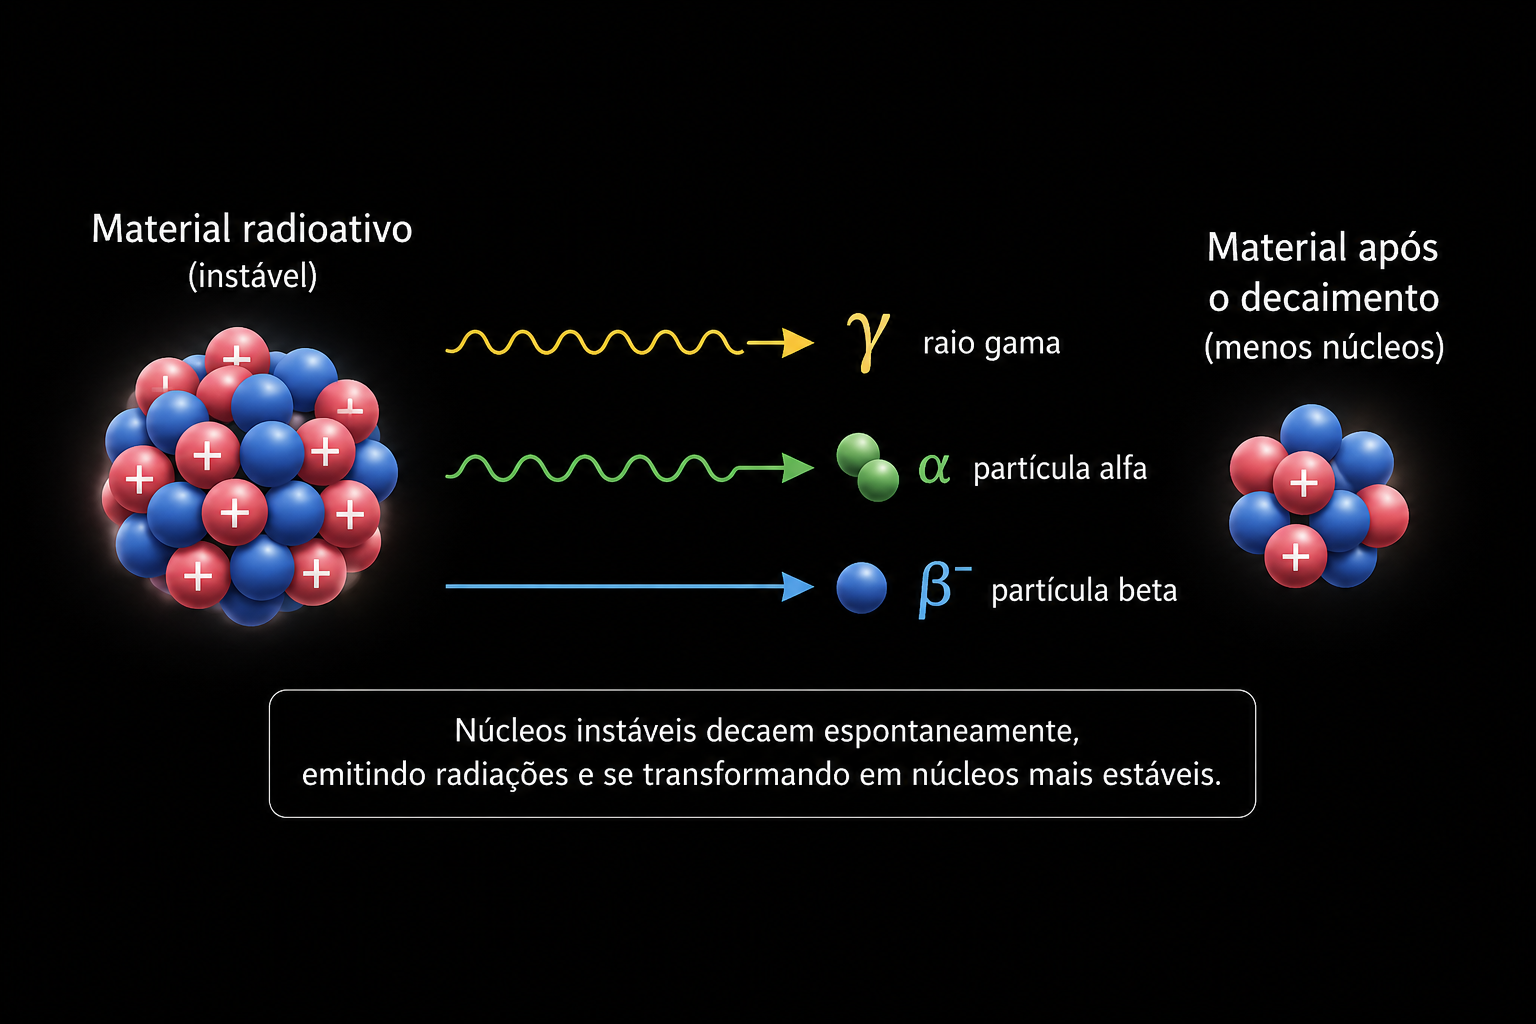
\includegraphics[width=\linewidth]{figuras/decaimento_radioativo.png}

\vspace{0.2cm}
\scriptsize
Fonte: Elaborado pelo Autor (2026)
\end{center}
\end{column}

%--------------------------------------------------
\begin{column}{0.58\textwidth}

A taxa de decaimento é proporcional à quantidade de núcleos radioativos presentes:

\[
\frac{dN}{dt}=-\lambda N,
\]

em que:

\begin{itemize}
    \item $N(t)$ é a quantidade de núcleos radioativos no instante $t$;
    \item $\lambda>0$ é a constante de decaimento;
    \item quanto maior $N(t)$, maior é a taxa de decaimento.
\end{itemize}

A solução da EDO é $N(t)=N_0e^{-\lambda t}$
\end{column}

\end{columns}
\end{frame}

% ===================== 2.2 LEI DE HOOKE =====================
\begin{frame}{2.2 Exemplo: Lei de Hooke}
\begin{columns}[T]

%--------------------------------------------------
\begin{column}{0.42\textwidth}
\begin{center}
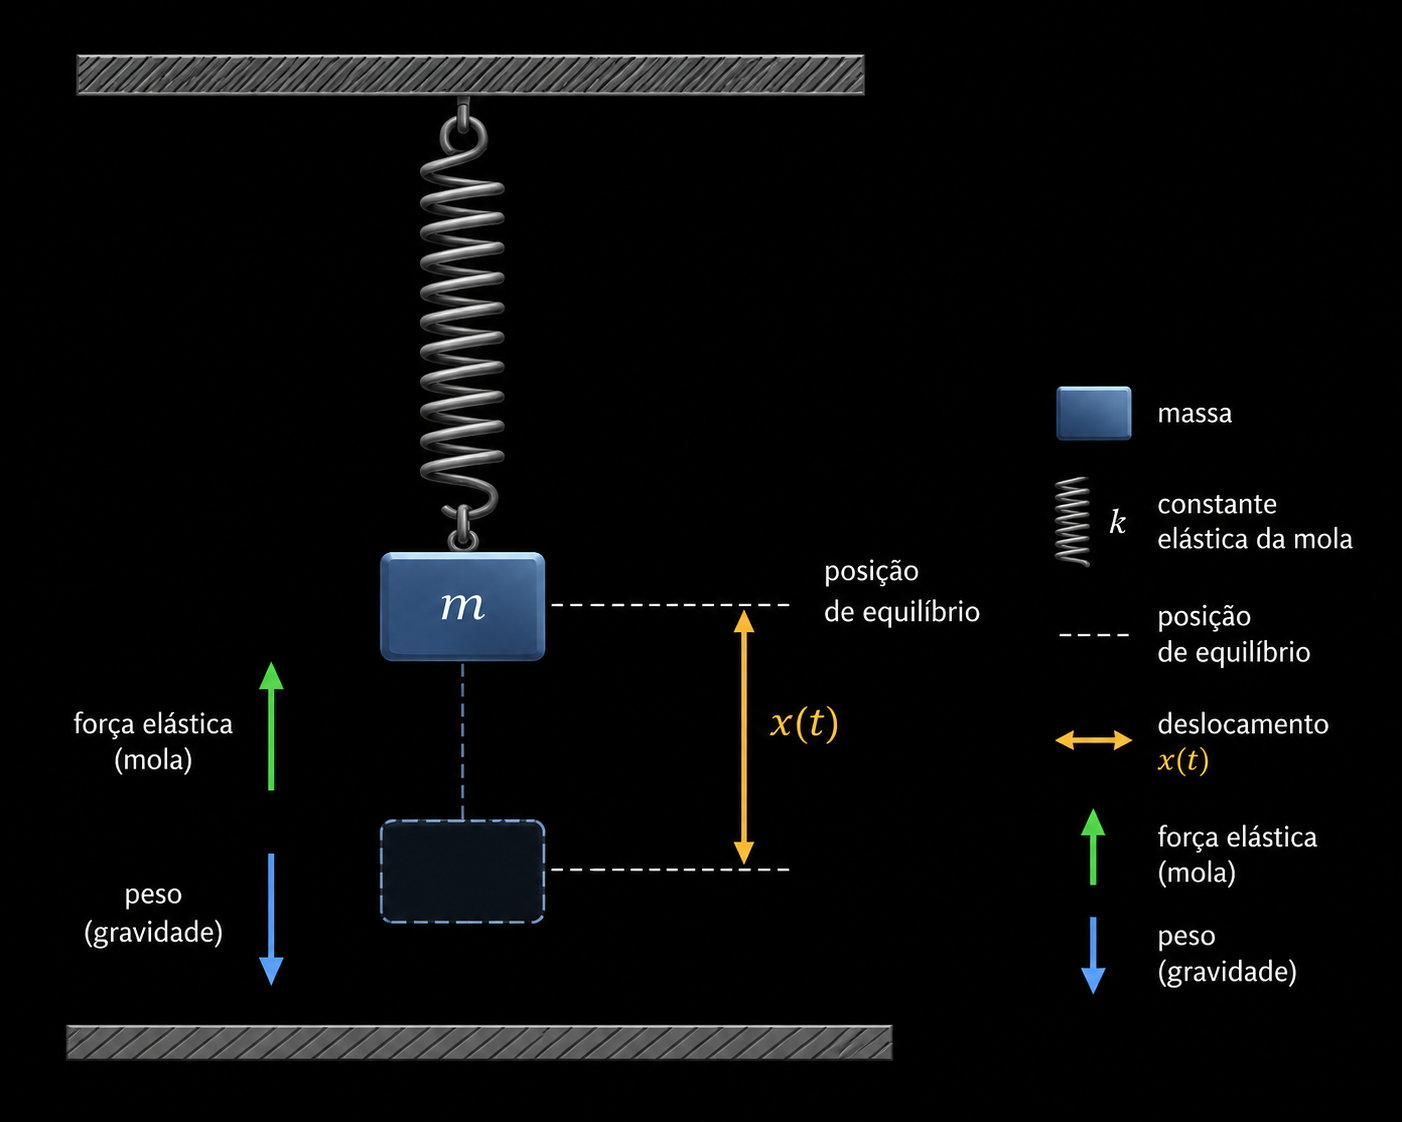
\includegraphics[width=0.90\linewidth]{figuras/lei_hooke.png}

\vspace{0.2cm}
\scriptsize
Fonte: Elaborado pelo Autor (2026)
\end{center}
\end{column}

%--------------------------------------------------
\begin{column}{0.58\textwidth}

A força restauradora da mola é dada pela Lei de Hooke é $F=-kx$. Onde:

\begin{itemize}
    \item $k>0$ é a constante elástica;
    \item $x(t)$ é o deslocamento da massa.
\end{itemize}

Pela Segunda Lei de Newton, temos:

\[
F=m\frac{d^{2}x}{dt^{2}}.
\]

Logo; $m\frac{d^{2}x}{dt^{2}}=-kx$

obtendo uma EDO de segunda ordem que descreve o movimento oscilatório.

\end{column}

\end{columns}
\end{frame}

% ===================== 3. TERMINOLOGIA =====================
\begin{frame}{3. Terminologia Fundamental: Ordem}

\vspace{0.2cm}
A \textbf{ordem} de uma EDO é a \textbf{maior derivada} que aparece na equação.

\vspace{0.3cm}
\begin{center}
\large
\begin{tabular}{lc}
\textcolor{accent}{\textbf{Equação}} & \textcolor{accent}{\textbf{Ordem}} \\
\hline
$y' = 2x$ & 1ª \\
$y'' + 3y' - y = 0$ & 2ª \\
$y''' = \sin(x)$ & 3ª \\
\end{tabular}
\end{center}
\end{frame}

\begin{frame}{3.2. Terminologia Fundamental: Grau}
O \textbf{grau} de uma EDO é a \textbf{potência} em que a derivada de maior ordem aparece, desde que a equação seja \textbf{polinomial} nas derivadas (sem raízes nem frações envolvendo derivadas).

\textbf{Exemplos:}
\begin{itemize}
  \item $y'' + y = 0$ $\rightarrow$ grau \textbf{1} (pois $y''$ aparece elevado à 1ª potência)
  \item $(y'')^3 + y = x$ $\rightarrow$ grau \textbf{3}
  \item $\sqrt{y''} + y = 0$ $\rightarrow$ grau \textbf{indefinido} (não é polinomial em $y''$)
\end{itemize}
\end{frame}

\begin{frame}{3.3 Linearidade}
Uma EDO de ordem $n$ é \textbf{linear} se puder ser escrita na forma:
\[
a_n(x)\,y^{(n)} + a_{n-1}(x)\,y^{(n-1)} + \cdots + a_1(x)\,y' + a_0(x)\,y = g(x)
\]

Exigências para linearidade:
\begin{enumerate}
  \item $y$ e todas as suas derivadas aparecem apenas com \textbf{potência 1}
  \item Não há \textbf{produtos} entre $y$ e suas derivadas
  \item Os coeficientes $a_k(x)$ dependem apenas de $x$
\end{enumerate}

Se qualquer dessas condições falha, a EDO é \textbf{não linear}.
\end{frame}

\begin{frame}{3.4 Homogeneidade}
Para EDOs lineares da forma $a_n(x)y^{(n)} + \cdots + a_0(x)y = g(x)$:

\begin{itemize}
  \item \textbf{Homogênea:} $g(x) = 0$ para todo $x$
  \[
    y'' + 3y' - y = 0
  \]
  \item \textbf{Não homogênea:} $g(x) \neq 0$
  \[
    y'' + 3y' - y = e^x
  \]
\end{itemize}
\end{frame}

\begin{frame}{3.5 EDO Autônoma}
Uma EDO é \textbf{autônoma} quando a variável independente $x$ não aparece explicitamente:
\[
\frac{dy}{dx} = f(y)
\]

\textbf{Exemplo:} $\dfrac{dy}{dx} = y(1 - y)$

São especialmente importantes em modelos populacionais e físicos, pois o comportamento do sistema não depende do "instante de partida".
\end{frame}

% ===================== 4. EXEMPLOS E CLASSIFICAÇÃO =====================
\begin{frame}{4. Exemplos e Classificação}
\textbf{1. EDO de 1ª ordem, linear, homogênea:}
\[
\frac{dy}{dx} + p(x)\,y = 0
\]

\textbf{2. EDO de 1ª ordem, linear, não homogênea:}
\[
\frac{dy}{dx} + p(x)\,y = q(x)
\]
\end{frame}

\begin{frame}{4. Exemplos e Classificação (cont.)}
\textbf{3. EDO de 2ª ordem, linear, homogênea:}
\[
y'' + a(x)\,y' + b(x)\,y = 0
\]

\textbf{4. EDO não linear --- Equação de Bernoulli:}
\[
\frac{dy}{dx} + p(x)\,y = q(x)\,y^n, \quad n \neq 0, 1
\]
\textit{(não linear pois $y^n$ aparece com potência $n > 1$)}
\end{frame}

\begin{frame}{4. Exemplos e Classificação (cont.)}
\textbf{5. EDO autônoma não linear (modelo logístico):}
\[
\frac{dP}{dt} = r\,P\!\left(1 - \frac{P}{K}\right)
\]

\textbf{6. EDO não linear com derivada elevada ao quadrado:}
\[
(y')^2 + y = \sin x
\]
\end{frame}

% ===================== 5. O QUE É UMA SOLUÇÃO =====================
\begin{frame}{5. O que é uma Solução?}
Uma \textbf{solução} de uma EDO em um intervalo $I$ é uma função $\phi(x)$, definida e derivável em $I$, tal que ao substituí-la na equação, a igualdade é satisfeita \textbf{identicamente} em $I$.

\textbf{Exemplo:} Verifique que $y = e^{2x}$ é solução de $y' - 2y = 0$.
\begin{itemize}
  \item Calculamos: $y' = 2e^{2x}$
  \item Substituímos: $2e^{2x} - 2e^{2x} = 0$ \checkmark
\end{itemize}
\end{frame}

\begin{frame}{5.1 Família de Soluções}
Em geral, resolver uma EDO de ordem $n$ produz uma \textbf{família de soluções} com $n$ constantes arbitrárias $C_1, C_2, \ldots, C_n$:
\[
y' = 2x \;\Longrightarrow\; y = x^2 + C
\]
Cada valor de $C$ corresponde a uma curva diferente --- chamamos esse conjunto de \textbf{solução geral}.
\end{frame}

\begin{frame}{5.2 Problema de Valor Inicial (PVI)}
Para selecionar \textbf{uma solução específica} dentro da família, impomos \textbf{condições iniciais}: valores de $y$ (e possivelmente de $y'$, $y''$, \ldots) em um ponto $x_0$.

\textbf{Exemplo:}
\[
y' = 2x, \quad y(1) = 3
\]
\begin{itemize}
  \item Solução geral: $y = x^2 + C$
  \item Usando $y(1) = 3$: $3 = 1 + C \Rightarrow C = 2$
  \item \textbf{Solução particular:} $y = x^2 + 2$
\end{itemize}
\end{frame}

\begin{frame}{5.3 Solução Explícita e Implícita}
\begin{itemize}
  \item \textbf{Explícita:} $y$ está isolada: $y = x^2 + 2$
  \item \textbf{Implícita:} a solução é dada por uma relação $G(x, y) = 0$, sem que $y$ esteja isolada:
  \[
    x^2 + y^2 = 1
  \]
\end{itemize}
Nem sempre é possível ou conveniente isolar $y$ --- soluções implícitas são perfeitamente válidas.
\end{frame}

\begin{frame}{5.4 Existência e Unicidade (Intuição)}
Uma pergunta natural: \textbf{toda EDO tem solução? E ela é única?}

O \textbf{Teorema de Picard--Lindelöf} garante que, sob condições de regularidade em $f(x,y)$, o PVI
\[
y' = f(x,y), \quad y(x_0) = y_0
\]
possui \textbf{solução única} em algum intervalo ao redor de $x_0$.

\notebox{Não provaremos o teorema, mas é importante saber que nem toda EDO tem solução, e nem toda solução é única.}
\end{frame}

% ===================== 6. EDOs EM MODELOS MATEMÁTICOS =====================
\begin{frame}{6. EDOs em Modelos Matemáticos}
\textbf{Crescimento exponencial (Malthus, 1798):}
\[
\frac{dP}{dt} = r\,P, \quad P(0) = P_0
\]
Solução: $P(t) = P_0\,e^{rt}$.

\vspace{0.3cm}

\textbf{Resfriamento de Newton:}
\[
\frac{dT}{dt} = -k\,(T - T_{\text{amb}})
\]
Descreve como a temperatura de um objeto se aproxima da temperatura ambiente.
\end{frame}

\begin{frame}{6. EDOs em Modelos Matemáticos (cont.)}
\textbf{Circuito RC (resistor-capacitor):}
\[
R\,\frac{dq}{dt} + \frac{q}{C} = V(t)
\]
Relaciona a carga $q(t)$ no capacitor com a tensão aplicada $V(t)$.

\notebox{Perceba que \textbf{resolver} a EDO significa encontrar a função que descreve o fenômeno.}
\end{frame}

% ===================== 7. EXERCÍCIOS DE FIXAÇÃO =====================
\begin{frame}{7. Exercícios de Fixação}
1) Para cada EDO abaixo, identifique: ordem, grau (se definido), linear ou não linear, homogênea ou não (quando aplicável).
\begin{itemize}
  \item[a)] $y'' + 5y' - 6y = \cos x$
  \item[b)] $\bigl(y'\bigr)^2 + y = x$
  \item[c)] $y''' - y'' + y = 0$
  \item[d)] $y' = y^2 - x$
\end{itemize}
\end{frame}

\begin{frame}{7. Exercícios de Fixação (cont.)}
2) Verifique se as funções dadas são soluções das respectivas EDOs.
\begin{itemize}
  \item[a)] $y = 3e^{-x}$ é solução de $y' + y = 0$?
  \item[b)] $y = \sin(2x)$ é solução de $y'' + 4y = 0$?
  \item[c)] $y = x\ln x$ é solução de $x^2 y'' - xy' + y = 0$?
\end{itemize}
\end{frame}

\begin{frame}{7. Exercícios de Fixação (cont.)}
3) Resolva o que cada item pede.
\begin{itemize}
  \item[a)] Ache a solução geral de $y' = 3x^2$.
  \item[b)] Determine a constante usando $y(0) = 5$.
  \item[c)] Verifique sua resposta substituindo na EDO.
\end{itemize}
\end{frame}

\begin{frame}{7. Exercícios de Fixação (cont.)}
4) Considere o modelo de resfriamento de Newton:
\[
\frac{dT}{dt} = -k\,(T - 20), \quad k > 0
\]
onde $T$ é a temperatura (em °C) e $t$ é o tempo (em minutos), sendo 20°C a temperatura ambiente.
\begin{itemize}
  \item[a)] Que tipo de EDO é essa (ordem, linearidade)?
  \item[b)] Interprete fisicamente o sinal negativo no lado direito.
  \item[c)] Se a temperatura inicial é $T(0) = 80\,^\circ\text{C}$, qual seria o comportamento esperado de $T(t)$ quando $t \to \infty$?
\end{itemize}
\end{frame}

% ===================== 8. ROTEIRO DE RESOLUÇÕES =====================
\begin{frame}{8. Roteiro de Resoluções}
\textbf{Exercício 1:}

\begin{center}
\small
\begin{tabular}{lccl}
\textcolor{accent}{\textbf{EDO}} & \textcolor{accent}{\textbf{Ordem}} & \textcolor{accent}{\textbf{Grau}} & \textcolor{accent}{\textbf{Tipo}} \\
\hline
a) $y'' + 5y' - 6y = \cos x$ & 2ª & 1 & Linear, NH \\
b) $(y')^2 + y = x$ & 1ª & 2 & Não linear \\
c) $y''' - y'' + y = 0$ & 3ª & 1 & Linear, H \\
d) $y' = y^2 - x$ & 1ª & 1 & Não linear \\
\end{tabular}
\end{center}
\end{frame}

\begin{frame}{8. Roteiro de Resoluções (cont.)}
\textbf{Exercício 2a:} $y = 3e^{-x}$, EDO: $y' + y = 0$

$y' = -3e^{-x} \;\Longrightarrow\; y' + y = -3e^{-x} + 3e^{-x} = 0$ \checkmark

\vspace{0.4cm}
\textbf{Exercício 2b:} $y = \sin(2x)$, EDO: $y'' + 4y = 0$

$y' = 2\cos(2x),\; y'' = -4\sin(2x)$

$y'' + 4y = -4\sin(2x) + 4\sin(2x) = 0$ \checkmark
\end{frame}

\begin{frame}{8. Roteiro de Resoluções (cont.)}
\textbf{Exercício 3:}
\begin{itemize}
  \item[a)] $y' = 3x^2 \;\Longrightarrow\; y = x^3 + C$ (solução geral)
  \item[b)] $y(0) = 5 \;\Longrightarrow\; 5 = 0 + C \;\Longrightarrow\; C = 5$ \\
  Solução particular: $y = x^3 + 5$
  \item[c)] Verificação: $y' = 3x^2$ \checkmark
\end{itemize}
\end{frame}

% ===================== 9. CONEXÃO COM A PRÓXIMA AULA =====================
\begin{frame}{9. Conexão com a Próxima Aula}
Agora que conhecemos os conceitos fundamentais das EDOs, estamos prontos para \textbf{resolver} equações de primeira ordem.

\textbf{Aula 02 --- Capítulo 2:} EDOs de Primeira Ordem
\begin{itemize}
  \item Método de \textbf{separação de variáveis}
  \item Equações \textbf{lineares de 1ª ordem} e o fator integrante
  \item Equações de \textbf{Bernoulli}
  \item Aplicações: modelos de crescimento, decaimento, misturas
\end{itemize}
\end{frame}

% ===================== 10. REFERÊNCIAS =====================
\begin{frame}{10. Referências}
\small
\begin{itemize}
  \item OLIVEIRA, Rafael Lima. \textit{Equações diferenciais ordinárias: métodos de resolução e aplicações.} Curitiba: Intersaberes, 2019.
  \item IANA, Marcelo. \textit{Mestrado: Equações Diferenciais Ordinárias}. Instituto de Matemática Pura e Aplicada (IMPA), YouTube, 15 mar. 2022.  Disponível em: \url{https://www.youtube.com/watch?v=wVp10rmsch0}.  Acesso em: 21 jul. 2026.
  \item UNIVERSIDADE ESTADUAL DE LONDRINA (UEL). \textit{Equações diferenciais ordinárias.} Disponível em: \url{http://www.uel.br/projetos/matessencial/superior/pdfs/edo.pdf}.
\end{itemize}
\end{frame}

\end{document}